%%%%%%%%%%%%%%%%%%%%%%%%%%%%%%%%%%%%%%%%%
% Template LaTeX Template Version 1.0 (December 8 2014)
%
% This template has been downloaded from: http://www.LaTeXTemplates.com
%
% Original author: Brandon Fryslie With extensive modifications by: Vel
% (vel@latextemplates.com)
%
% License: CC BY-NC-SA 3.0 (http://creativecommons.org/licenses/by-nc-sa/3.0/)
%
% Authors: Sabbir Ahmed, Jeffrey Osazuwa, Howard To, Brian Weber
% 
%%%%%%%%%%%%%%%%%%%%%%%%%%%%%%%%%%%%%%%%%

\documentclass[paper=usletter, fontsize=12pt]{extarticle}
%%%%%%%%%%%%%%%%%%%%%%%%%%%%%%%%%%%%%%%%%
% Contract Structural Definitions File Version 1.0 (December 8 2014)
%
% Created by: Vel (vel@latextemplates.com)
% 
% This file has been downloaded from: http://www.LaTeXTemplates.com
%
% License: CC BY-NC-SA 3.0 (http://creativecommons.org/licenses/by-nc-sa/3.0/)
%
%%%%%%%%%%%%%%%%%%%%%%%%%%%%%%%%%%%%%%%%%

\usepackage{geometry} % Required to modify the page layout
\usepackage{multicol}
\usepackage{amsmath}
\usepackage{amssymb}

\usepackage[pdftex]{graphicx}
\usepackage{wrapfig}
\usepackage[font=scriptsize, labelfont=bf]{caption}
\usepackage[utf8]{inputenc} % Required for including letters with accents
\usepackage[T1]{fontenc} % Use 8-bit encoding that has 256 glyphs

\usepackage{avant} % Use the Avantgarde font for headings
\usepackage{courier}
\usepackage{xparse}
\usepackage{xcolor}
\usepackage{listings}  % for code verbatim and console outputs

\setlength{\textwidth}{16cm} % Width of the text on the page
\setlength{\textheight}{23cm} % Height of the text on the page
\setlength{\oddsidemargin}{0cm} % Width of the margin - negative to move text left, positive to move it right
\setlength{\topmargin}{-1.25cm} % Reduce the top margin

\setlength{\parindent}{0mm} % Don't indent paragraphs
\setlength{\parskip}{2.5mm} % Whitespace between paragraphs
\renewcommand{\baselinestretch}{1.5}

\definecolor{green}{rgb}{0.18, 0.55, 0.34}

\graphicspath{ {figures/} }
\captionsetup[table]{skip=10pt}

\lstset{language=C, keywordstyle={\bfseries \color{black}}}

% defines algorithm counter for chapter-level
\newcounter{nalg}[section]

%defines appearance of the algorithm counter
\renewcommand{\thenalg}{\thesection .\arabic{nalg}}

% defines a new caption label as Algorithm x.y
\DeclareCaptionLabelFormat{algocaption}{Algorithm \thenalg}

% defines the algorithm listing environment
\lstnewenvironment{pseudocode}[1][] {
    \refstepcounter{nalg}  % increments algorithm number
    \captionsetup{font=normalsize, labelformat=algocaption, labelsep=colon}
    \lstset{
        breaklines=true,
        mathescape=true,
        numbers=left,
        numberstyle=\scriptsize,
        basicstyle=\footnotesize\ttfamily,
        keywordstyle=\color{black}\bfseries,
        keywords={input, output, return, parallel, function, for, to, in, if,
        else, foreach, while, and, or, new, print},
        xleftmargin=.04\textwidth,
        #1
    }
}{}

\renewcommand{\familydefault}{\sfdefault}  % default font for entire document
 % specifies the document layout and style

% document info command
\newcommand{\documentinfo}[5]{
    \begin{centering}
        \parbox{2in}{
        \begin{spacing}{1}
            \begin{flushleft}
                \begin{tabular}{l l} #1 \\ #2 \\ #3 \\
                \end{tabular}\\
                \rule{\textwidth}{1pt}
            \end{flushleft}
        \end{spacing} }
    \end{centering} }
\renewcommand{\baselinestretch}{1.5}  % space between lines

\begin{document}


    \documentinfo{Final Exams: Extra Credit Code Snippet}{Sabbir Ahmed}{Date:
    \today}
    \vspace{-0.1in}

    \section{More Usefulness of \texttt{`printf()'}}
    \texttt{printf()} is one of the most useful functions for beginners in the
    C programming language. It is a very helpful tool when it comes to
    debugging, checking statuses of dynamic variables, or simply printing to
    console. What many users are unaware of is that the function may be used
    for other very useful tricks. Like the last code snippet, here are some
    additional tricks with \texttt{printf()}.

    \subsection{\%m Specifier}

    The following snippet will print out ``Success''.

\begin{lstlisting}
#include <stdio.h>
int main() {
    printf("%m");
    return 0;
}
\end{lstlisting}

    \begin{figure}[ht]
        \begin{center}
            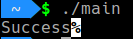
\includegraphics[width=0.25\textwidth]{build1.png}
            \caption{Running Snippet 1} \label{fig:build1}
        \end{center}
    \end{figure}

    \texttt{\%m} only prints “Success” when \texttt{“errno == 0”}. It is short
    for a string representation of the last observed error state. For instance,
    if a function fails before the \texttt{printf()}, it will print something
    rather different. Therefore, the snippet is equivalent to the following
    line:

\begin{lstlisting}
#include <stdio.h>
int main() {
    printf("%s\n", strerror (errno));
    return 0;
}
\end{lstlisting}

    Note that the \texttt{\%m} specifier is a GNU C extension of
    \texttt{printf()}.

    \subsection{`*' Specifier}

    Another feature with the format specifiers is that the asterisk character
    (*) may be used to format the specifiers with variables. For example, the
    following snippet:

\begin{lstlisting}
#include <stdio.h>
int main() {
    int sig_fig = 4;
    double pi = 3.14159265358979323846;
    printf("%.*f\n", sig_fig, pi);
    return 0;
}
\end{lstlisting}

    will generate the following output:

    \begin{figure}[ht]
        \begin{center}
            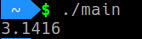
\includegraphics[width=0.25\textwidth]{build2.png}
            \caption{Running Snippet 2} \label{fig:build2}
        \end{center}
    \end{figure}

    Since \texttt{sig\_fig} was 4, the \texttt{\%.*f} specifier printed the
    value of pi to 4 significant figures.


\end{document}
